\documentclass[a4paper,11pt]{article}

\newcommand{\CurrentVersion}{2.0.0} % ultima versione, da cambiare ad ogni push significativo

\usepackage[utf8]{inputenc}
\usepackage[T1]{fontenc}
\usepackage[italian]{babel}
\usepackage[margin=2.5cm]{geometry}
\usepackage{graphicx}
\usepackage{grffile}
\usepackage{booktabs}
\usepackage{setspace}
\usepackage{titlesec}
\usepackage{float}
\usepackage{ifthen}
\usepackage[table]{xcolor}
\usepackage{tabularx}
\usepackage{needspace}
\usepackage{tcolorbox}
\usepackage{enumitem}
\usepackage[titles]{tocloft}
\usepackage[colorlinks=true,linkcolor=black,urlcolor=blue,citecolor=blue]{hyperref}
\usepackage{xspace}
% Macro
\input{../../assets/macro/macro-verbali.tex}

\definecolor{primaryblue}{RGB}{0,102,204}
\definecolor{secondaryblue}{RGB}{51,153,255}
\definecolor{lightgray}{RGB}{245,245,245}
\definecolor{darkgray}{RGB}{100,100,100}

\titleformat{\section}
 {\Large\bfseries\color{primaryblue}}
 {\thesection}{1em}{}

\titleformat{\subsection}
 {\large\bfseries\color{primaryblue}} % Sottosezione: colore secondaryblue
 {\thesubsection}{1em}{}

\titleformat{\subsubsection}
 {\normalsize\bfseries\color{secondaryblue}} % Sotto-sottosezione: colore secondaryblue
 {\thesubsubsection}{1em}{}

% per il footer con il numero di pagina
\usepackage{fancyhdr}
\usepackage{lastpage} % per ottenere il numero dell'ultima pagina da mettere nel footer

\usepackage{ltablex} %per far andare a capo le tabelle
\keepXColumns

\renewcommand{\sectionmark}[1]{\markright{#1}}
\renewcommand{\G}{\texorpdfstring{\textsubscript{\scalebox{0.6}{\textbf{G}}}\xspace}{ G}}

% Macro tabella metrica (tabella uniforme, non spezzata e con stile coerente)
\newcommand{\MetricTable}[1]{
  \Needspace{10\baselineskip}% evita spezzamenti sgradevoli
  \begin{table}[H]
  \centering
  \arrayrulecolor{primaryblue}
  \begin{tabularx}{\linewidth}{|>{\raggedright\arraybackslash}p{2.5cm}|X|>{\raggedright\arraybackslash}p{3cm}|>{\raggedright\arraybackslash}p{3cm}|}
  \hline
  \rowcolor{primaryblue!40}
      \textbf{\color{white} Metrica} & \textbf{\color{white} Descrizione} & \textbf{\color{white} Valore accettazione} & \textbf{\color{white} Valore ideale} \\
  \hline
  \ignorespaces
  #1
  \end{tabularx}
  \end{table}
}



\setlength{\parskip}{4pt}
\setlength{\parindent}{0pt}

\setlist[itemize]{leftmargin=*,itemsep=3pt}
\setlist[enumerate]{leftmargin=*,itemsep=3pt}

\graphicspath{{./}{../assets/images/}{./images/}}

\begin{document}

%configurazione per il footer
\pagestyle{fancy}
\fancyhf{} % pulisce tutti i campi del header e footer
\setlength{\headheight}{14pt}

% Header: sinistra e destra
\fancyhead[L]{Gruppo 4 - BugBusters} % sinistra
\fancyhead[R]{Piano di Qualifica\G}   % destra

\fancyfoot[L]{ \thepage\ di \pageref{LastPage}} %definisce il formato del footer
\fancyfoot[R]{ \nouppercase{\rightmark}} % nome della sezione


\renewcommand{\headrulewidth}{0pt} % rimuove la linea dell'header
\renewcommand{\footrulewidth}{0pt} % se vuoi anche togliere eventuale linea del footer

% abilitare numerazione e TOC fino al livello "paragraph" (subsubsubsection)
\setcounter{secnumdepth}{4}
\setcounter{tocdepth}{4}
% formattazione del nuovo livello per avere aspetto coerente
\titleformat{\paragraph}[block]{\normalsize\bfseries\color{secondaryblue}}{\theparagraph}{1em}{}
% alias comodo per usare "subsubsubsection"
\newcommand{\subsubsubsection}{\paragraph}

\begin{center}
  \IfFileExists{../../assets/Logo.jpg}{%
    
\includegraphics[width=6cm,height=3cm,keepaspectratio]{../../assets/Logo.jpg} \\[0.8cm]
  }{%
    \fbox{\parbox[c][2.5cm][c]{6cm}{\centering Logo non trovato\\(../../assets/Logo.jpg)}}\\[0.5cm]
  }
  
  {\Large\bfseries\color{primaryblue} BugBusters}\\[0.5cm]

  {\Huge\bfseries\color{primaryblue} Piano di Qualifica\G}\\[0.3cm]
  {\Large\color{secondaryblue} Versione \CurrentVersion}\\[0.8cm]
\end{center}

\begin{center}
\begin{tcolorbox}[colback=lightgray,colframe=primaryblue,width=0.85\textwidth,arc=3mm,boxrule=0.5pt]
% Usa tabularx con una colonna fissa per l'etichetta e una colonna X per il contenuto
\begin{tabularx}{\linewidth}{@{}>{\raggedright\arraybackslash}p{3.5cm}>{\raggedright\arraybackslash}X@{}}
  {Stato} & Approvato \\
  {Redattori\G} & Marco Favero, Linor Sadé, Marco Piro, Leonardo Salviato \\
  {Verificatori\G} & Alberto Pignat, Marco Favero, Linor Sadè \\
  {Distribuzione} & BugBusters, Eggon, Prof. Tullio Vardanega, Prof. Riccardo Cardin \\
\end{tabularx}
\end{tcolorbox}
\end{center}

\vspace{0.5cm}

\begin{center}
\begin{tcolorbox}[colback=secondaryblue!10,colframe=secondaryblue,width=0.9\textwidth,arc=3mm,boxrule=0.8pt,title={\bfseries Descrizione}]
Piano di Qualifica\G del Team BugBusters per il Capitolato\G C5 proposto da Eggon, che ha l'obiettivo di far rispettare uno standard di qualità\G per il codice e rispettare i requisiti funzionali\G prestabiliti.\end{tcolorbox}
\end{center}

\newpage

% Registro delle Modifiche (pagina 2)
\section*{Registro delle Modifiche}

\arrayrulecolor{primaryblue}
{\footnotesize
\begin{tabularx}{\textwidth}{|>{\raggedright\arraybackslash}p{1.5cm}|>{\raggedright\arraybackslash}p{2cm}|X|>{\raggedright\arraybackslash}p{2cm}|>{\raggedright\arraybackslash}p{2cm}|>{\raggedright\arraybackslash}p{2cm}|}
\hline
\rowcolor{primaryblue!40}
\textbf{\color{white} Versione} & \textbf{\color{white} Data} & \textbf{\color{white} Descrizione} & \textbf{\color{white} Redatto} & \textbf{\color{white} Verificato} & \textbf{\color{white} Approvato} \\
\hline
\rowcolor{secondaryblue!10}2.0.0 & 03/04/2026 & Approvazione\G documento & - & - & Linor Sadè \\
\hline
\rowcolor{secondaryblue!10}1.2.0 & 03/04/2026 & Verifica\G documento & - & Alberto Pignat & - \\
\hline
\rowcolor{secondaryblue!10}1.1.1 & 03/04/2026 & Conclusione documento & Marco Piro & - & - \\
\hline
\rowcolor{secondaryblue!10}1.1.0 & 28/02/2026 & Verifica\G documento & - & Linor Sadè & - \\
\hline
\rowcolor{secondaryblue!10}1.0.1 & 26/02/2026 & Correzione post valutazione RTB\G & Marco Piro & - & - \\
\hline
\rowcolor{secondaryblue!10}1.0.0 & 08/02/2026 & Effettuata approvazione\G & - & - & Luca Slongo \\
\hline
\rowcolor{secondaryblue!10}0.2.0 & 08/02/2026 & Effettuata verifica\G & - & Marco Favero & - \\
\hline
\rowcolor{secondaryblue!10}0.1.4 & 01/02/2026 & Aggiunti ai termini presenti nel Glossario\G la G & Luca Slongo & - & - \\
\hline
\rowcolor{secondaryblue!10}0.1.3 & 01/02/2026 & Aggiunta descrizione grafici metriche & Leonardo Salviato & - & - \\
\hline
\rowcolor{secondaryblue!10}0.1.2 & 04/02/2026 & Aggiunti grafici metriche, aggiornamento Test\G, rimossa matrice di Tracciamento & Leonardo Salviato & - & - \\
\hline
\rowcolor{secondaryblue!10}0.1.1 & 19/01/2026 & Aggiornamento Test\G, aggiunti test\G di sistema Casi Limite e integrazione, cambiato alcune metriche di prodotto\G. Aggiunta matrice di Tracciamento & Linor Sadé & - & - \\
\hline
\rowcolor{secondaryblue!10}0.1.0 & 16/01/2026 & Verifica\G intermedia & - & Alberto Pignat & - \\
\hline
\rowcolor{secondaryblue!10}0.0.5 & 15/01/2026 & Aggiornamento Test\G, aggiunti test\G di sistema prestazionali, eliminata metrica errori ortografici & Linor Sadé & - & - \\
\hline
\rowcolor{secondaryblue!10}0.0.4 & 11/01/2026 & Aggiunto contenuto alla sezione 5 & Linor Sadé & - & - \\
\hline
\rowcolor{secondaryblue!10}0.0.3 & 04/01/2026 & Aggiunte sezioni 4 e 5 & Marco Piro & - & - \\
\hline
\rowcolor{secondaryblue!10}0.0.2 & 29/12/2025 & Aggiunta Test\G di Sistema e di Accettazione & Marco Piro & - & - \\
\hline
\rowcolor{secondaryblue!10}0.0.1 & 03/12/2025 & Prima stesura del documento & Marco Favero & - & - \\
\hline
\end{tabularx}
}

\newpage

% Indice cliccabile
\setcounter{tocdepth}{3} % Mostra fino al livello di sottosezione (2)
\tableofcontents
\listoftables
\listoffigures

\newpage
\section{Introduzione}

\subsection{Scopo del documento}
Il presente documento, denominato \textit{Piano di Qualifica\G}, ha lo scopo di definire le strategie, le procedure e le metriche adottate dal gruppo \textit{BugBusters} per garantire la qualità\G del prodotto\G software e dei processi produttivi relativi al progetto\G C5 (NEXUM), proposto dall'azienda \textit{Eggon}.

In particolare, questo documento si prefigge di:
\begin{itemize}
    \item \textbf{Definire gli obiettivi di qualità\G:} specificare i target qualitativi per il processo di sviluppo (efficienza\G, stabilità) e per il prodotto\G software (funzionalità\G, affidabilità\G, manutenibilità\G), in conformità con gli standard ISO/IEC 12207 e ISO/IEC 9126;
    \item \textbf{Identificare le metriche:} selezionare gli indicatori quantitativi più idonei per monitorare il raggiungimento degli obiettivi, fissando per ciascuno le soglie di accettazione e di ottimalità;
    \item \textbf{Pianificare le attività di verifica\G e validazione\G:} descrivere le metodologie di test\G (unità, integrazione, sistema, accettazione) e le procedure di analisi statica del codice e della documentazione;
    \item \textbf{Monitorare l'andamento del progetto\G:} fornire un resoconto puntuale (cruscotto\G di valutazione) delle misurazioni effettuate durante le varie fasi del ciclo di vita, permettendo al team di individuare tempestivamente criticità e attuare azioni correttive (miglioramento continuo).
\end{itemize}

\subsection{Glossario\G}
Al fine di evitare ambiguità e garantire una comprensione uniforme della terminologia utilizzata, è stato redatto un documento esterno denominato \textit{Glossario\G}.
I termini tecnici, gli acronimi e le parole con un significato specifico all'interno del progetto\G sono contrassegnati nel testo da una "G" in pedice (es. parola). La loro definizione completa è consultabile nel \textit{Glossario\G}.

\subsection{Riferimenti}

\subsubsection{Riferimenti normativi}
\begin{itemize}
    \item \textbf{Capitolato\G d'appalto C5 - NEXUM (Eggon):}\\
    \url{https://www.math.unipd.it/~tullio/IS-1/2025/Progetto/C5.pdf}
    
    \item \textbf{Norme di Progetto\G (v2.0.0):}\\
    Documento interno del gruppo \textit{BugBusters} che definisce le regole, i ruoli e le procedure operative.\\
    \url{https://bugbustersunipd.github.io/DocumentazioneSWE/PB/NORME%20DI%20PROGETTO/Norme%20di%20Progetto.pdf}
    
    \item \textbf{Regolamento del progetto\G didattico:} \\
    \url{https://www.math.unipd.it/~tullio/IS-1/2025/Dispense/PD1.pdf}
\end{itemize}

\subsubsection{Riferimenti informativi}
\begin{itemize}
    \item \textbf{Glossario\G (v2.0.0):}\\
    Documento interno del gruppo \textit{BugBusters} contenente le definizioni dei termini tecnici.\\
    \url{https://bugbustersunipd.github.io/DocumentazioneSWE/PB/GLOSSARIO/Glossario.pdf}
    \item \textbf{Standard ISO/IEC 12207:1995:}\\
    \textit{Information technology - Software life cycle processes}.\\
    \url{https://www.math.unipd.it/~tullio/IS-1/2009/Approfondimenti/ISO_12207-1995.pdf}
    
    \item \textbf{Standard ISO/IEC 9126:}\\
    \textit{Software engineering - Product quality}.\\
    \url{https://it.wikipedia.org/wiki/ISO/IEC_9126}
    
    \item \textbf{Slide del corso di Ingegneria del Software:} \\
    Materiale didattico fornito dai docenti Prof. Tullio Vardanega e Prof. Riccardo Cardin.
\end{itemize}
\newpage

\section{Obiettivi stabiliti per la qualità\G}

È fondamentale stabilire degli obiettivi da raggiungere per assicurare la qualità\G prefissata del prodotto\G. 
Questo documento definisce i valori di accettazione e ottimalità delle metriche secondo gli standard definiti 
nelle Norme di Progetto\G.

\subsection{Qualità\G di processo}
Un indicatore della qualità\G di un prodotto\G è il metodo con cui è stato sviluppato. Se il processo di sviluppo segue 
delle linee guida ben definite, esso favorisce la buona riuscita del prodotto\G. Come stabilito nelle Norme di Progetto\G, 
nel nostro way of working\G abbiamo adottato lo Standard ISO/IEC 12207:1995 adattandolo alle nostre esigenze e a quelle 
del progetto\G. 

\subsubsection{Processi primari}

I processi primari sono quelle attività che iniziano o eseguono lo sviluppo, l'operazione o la manutenzione di prodotti software. Essi rappresentano le componenti fondamentali del ciclo di vita del progetto\G e sono suddivisi nelle seguenti categorie:
\subsubsubsection{Fornitura}

\MetricTable{
MPC01 & Earned value (EV)\G & $\geq 0$ & $\leq$ EAC\G \\
\hline
MPC02 & Planned value (PV)\G & $\geq 0$ & $\leq$ Budget at completion (BAC) \\
\hline
MPC03 & Actual cost (AC)\G & $\geq 0$ & $\leq$ EAC\G \\
\hline
MPC04 & Cost Performance Index (CPI)\G & $\geq 0.9$ & 1 \\
\hline
MPC05 & Schedule Performance Index (SPI)\G & $\geq 0.9$ & 1 \\
\hline
MPC06 & Estimated at completion (EAC)\G & $\pm 5\%$ rispetto al (BAC) & Budget at completion (BAC) \\
\hline
MPC07 & Estimate to complete (ETC)\G & $\geq 0$ & $\leq$ EAC\G \\
\hline
MPC08 & Time Estimate At Completion (TEAC)\G & $\geq 0$ & $\leq$ Durata pianificata \\
\hline}



\subsubsubsection{Sviluppo}
\MetricTable{
MPC09 & Requirements Stability Index\G & $\geq 70\%$ & 100\% \\
\hline}


\subsubsection{Processi di supporto}
\subsubsubsection{Documentazione}
\MetricTable{
MPC10 & Indice di Gulpease\G del documento & $\geq 60\%$ & $\geq 80\%$ \\
\hline
}
\subsubsubsection{Verifica\G}
\MetricTable{
MPC11 & Code Coverage\G & $\geq 80\%$ & $100\%$ \\
\hline
MPC12 & Test\G Success Rate & $100\%$ & $100\%$ \\
\hline}
\subsubsubsection{Gestione della qualità\G}
\MetricTable{
MPC13 & Quality metrics satisfied & $\geq 80\%$ & $100\%$ \\
\hline}

\subsubsection{Processi organizzativi}
\subsubsubsection{Gestione dei processi}
\MetricTable{
MPC14 & Time Efficiency & $\geq 50\%$ & $100\%$ \\
\hline}



\subsection{Qualità\G di prodotto\G}

Per qualità\G di prodotto\G si intende una valutazione complessiva del software sia dal punto di vista 
funzionale sia dal punto di vista strutturale. Il codice deve adempiere alle funzionalità\G prestabilite in 
modo efficiente e semplice, e al contempo essere manutenibile, affidabile e portabile. Il gruppo ha aderito allo 
standard ISO/IEC 9126 per garantire il rispetto di queste caratteristiche fondamentali, affinché il prodotto\G 
sviluppato sia di alta qualità\G.

\subsubsection{Funzionalità\G}
\MetricTable{
MPD01 & Requisiti obbligatori\G soddisfatti & $100\%$ & $100\%$ \\
\hline
MPD02 & Requisiti desiderabili\G soddisfatti & $0\%$ & $100\%$ \\
\hline
MPD03 & Requisiti opzionali\G soddisfatti & $0\%$ & $100\%$ \\
\hline
MPD04 & AI\G Acceptance Rate (Rating $\geq$ 3/5) & $\geq 60\%$ & $\geq 80\%$ \\
\hline}

\subsubsection{Affidabilità\G}
\MetricTable{
MPD05 & Branch Coverage\G & $\geq 70\%$ & $\geq 85\%$ \\
\hline
MPD06 & Defect Density & $\leq 3$ / KLOC & $\leq 1$ / KLOC \\
\hline}

\subsubsection{Efficienza\G}
\MetricTable{
MPD07 & UI Response Time (Interfaccia\G) & $\leq 2$ sec & $\leq 0.5$ sec \\
\hline
MPD08 & Core Response Time - AI\G Generativo testo & $\leq 5$ sec & $\leq 3$ sec \\
\hline
MPD09 & Core Response Time - AI\G Generativo immagini & $\leq 10$ sec & $\leq 5$ sec \\
\hline
MPD10 & Core Response Time - AI Co-Pilot\G & $\leq 10$ sec & $\leq 5$ sec \\
\hline}

\subsubsection{Usabilità}
\MetricTable{
MPD11 & Click Count (Funzioni principali) & $\leq 5$ click & $\leq 3$ click \\
\hline
MPD12 & User Error Rate (Errori validazione\G) & $\leq 10\%$ & $\leq 5\%$ \\
\hline}

\subsubsection{Mantenibilità}
\MetricTable{
MPD13 & Blocker Code Smells & $0$ & $0$ \\
\hline
MPD14 & Cyclomatic complexity\G (per metodo) & $\leq 15$ & $\leq 10$ \\
\hline
MPD15 & Comment Intensity & $\geq 10\%$ & $\geq 20\%$ \\
\hline}

\subsubsection{Portabilità}
\MetricTable{
MPD16 & Supported Browsers (Test\G passati) & $100\%$ (Desktop) & $100\%$ (All devices) \\
\hline}



\section{Metodi di testing}
La strategia di verifica\G e validazione\G adottata dal gruppo \textit{BugBusters} mira a garantire che ogni rilascio software sia conforme ai requisiti specificati e privo di difetti critici.
I test\G dinamici pianificati seguono un approccio incrementale (piramide dei test\G), partendo dalle singole unità logiche fino alla validazione\G dell'intero sistema integrato.



\subsection{Test di Integrazione}
I test\G di integrazione verificano la corretta comunicazione tra i sottosistemi e i moduli definiti nell'architettura, assicurando che le interfacce e lo scambio dati avvengano come previsto.

\begin{longtable}{|p{2.2cm}|p{7cm}|p{3.5cm}|}
  \hline
  \rowcolor{primaryblue!30} 
  \textbf{Codice} & \textbf{Descrizione Interfaccia\G} & \textbf{Moduli Coinvolti} \\
  \hline
  \endhead
  
  \textbf{TI-001} & Verifica\G scambio dati e gestione errori tramite chiamate API\G REST (formato JSON). & Frontend\G (Angular\G) $\leftrightarrow$ Backend\G (Ruby on Rails\G) \\
  \hline
  \textbf{TI-002} & Verifica\G invio del contesto/prompt\G e ricezione dello stream di risposta dal servizio AI\G. & Backend\G (Assistant) $\leftrightarrow$ External LLM\G API\G \\
  \hline
  \textbf{TI-003} & Verifica\G dell'integrità dei dati salvati e recuperati (utenti, documenti, chat log). & Backend\G Logic $\leftrightarrow$ Database (PostgreSQL\G) \\
  \hline
  \textbf{TI-004} & Verifica\G del caricamento file, estrazione testo (OCR\G) e validazione\G formato. & Upload Service $\leftrightarrow$ PDF Parser Module \\
  \hline
  \textbf{TI-005} & Verifica\G dell'aggregazione dei dati per la generazione delle statistiche visualizzate nella dashboard\G. & Analytics Module $\leftrightarrow$ Database \\
  \hline
  \textbf{TI-006} & Verifica\G del sistema di autenticazione e gestione sessioni utente. & Auth Controller $\leftrightarrow$ Session Manager \\
  \hline
  
  \caption{Test di Integrazione}
  \label{tab:test-integrazione}
\end{longtable}


\subsection{Test\G di Sistema}

\subsubsection{Test\G di Sistema - Requisiti Funzionali}
\begin{longtable}{|p{2.2cm}|p{8.3cm}|p{2cm}|p{1.5cm}|}
\hline
\rowcolor{primaryblue!30} 
\textbf{Codice} & \textbf{Descrizione} & \textbf{Riferimento} & \textbf{Stato} \\
\hline
\endhead

% --- AUTENTICAZIONE E UTENTI (RF 1-25) ---
TS-F-001 & Verifica\G che il sistema permetta all'utente non autenticato di effettuare la registrazione. & RF-1 & NI \\ \hline
TS-F-002 & Verifica\G che il sistema permetta all'utente di inserire l'indirizzo email durante la registrazione. & RF-2 & NI \\ \hline
TS-F-003 & Verifica\G che il sistema permetta all'utente di inserire la password durante la registrazione. & RF-3 & NI \\ \hline
TS-F-004 & Verifica\G che il sistema permetta all'utente di inserire l'username durante la registrazione. & RF-4 & NI \\ \hline
TS-F-005 & Verifica\G che il sistema permetta all'utente di inserire il nome durante la registrazione. & RF-5 & NI \\ \hline
TS-F-006 & Verifica\G che il sistema permetta all'utente di inserire il cognome durante la registrazione. & RF-6 & NI \\ \hline
TS-F-007 & Verifica\G che il sistema permetta all'utente di inserire la propria matricola durante la registrazione. & RF-7 & NI \\ \hline
TS-F-008 & Verifica\G che il sistema permetta la visualizzazione di un errore se l'email non è valida. & RF-8 & NI \\ \hline
TS-F-009 & Verifica\G che il sistema permetta la visualizzazione di un errore se la password non rispetta i criteri di sicurezza\G. & RF-9 & NI \\ \hline
TS-F-010 & Verifica\G che il sistema impedisca la registrazione se
l’email inserita è già associata a un account
esistente. & RF-10 & NI \\ \hline
TS-F-011 & Verifica\G che il sistema impedisca la registrazione se
lo username inserito è già utilizzato. & RF-11 & NI \\ \hline
TS-F-012 & Verifica\G che il sistema impedisca la registrazione
se la matricola inserita è già presente nel
sistema. & RF-12 & NI \\ \hline
TS-F-013 & Verifica\G che il sistema permetta la visualizzazione di un messaggio
di errore se il formato della matricola non è
valido. & RF-13 & NI \\ \hline
TS-F-014 & Verifica\G che il sistema permetta all'utente di effettuare il login (autenticazione). & RF-14 & NI \\ \hline
TS-F-015 & Verifica\G che il sistema notifichi l’errore in caso di
tentativo di login con email non registrata o password associata all'email errata. & RF-15 & NI \\ \hline
TS-F-016 & Verifica\G che il sistema consenta all'utente di poter inserire i dati necessari al login. & RF-16 & NI \\ \hline
TS-F-017 & Verifica\G che il sistema permetta all'utente di visualizzare i dati del proprio profilo. & RF-17 & NI \\ \hline
TS-F-018 & Verifica\G che il sistema mostri l’email associata al
profilo utente. & RF-18 & NI \\ \hline
TS-F-019 & Verifica\G che il sistema mostri (o permetta la
gestione) della password del profilo utente. & RF-19 & NI \\ \hline
TS-F-020 & Verifica\G che il sistema mostri lo username
associato al profilo utente. & RF-20 & NI \\ \hline
TS-F-021 & Verifica\G che il sistema mostri il nome associato
al profilo utente. & RF-21 & NI \\ \hline
TS-F-022 & Verifica\G che il sistema mostri il cognome associato
al profilo utente. & RF-22 & NI \\ \hline
TS-F-023 & Verifica\G che il sistema mostri la matricola associata
al profilo utente. & RF-23 & NI \\ \hline
TS-F-024 & Verifica\G che il sistema permetta all'utente di effettuare il logout terminando la sessione. & RF-24 & NI \\ \hline
TS-F-025 & Verifica\G che il sistema gestisca l’uscita dalla modifica profilo senza salvare i
cambiamenti. & RF-25 & NI \\ \hline

TS-F-026 & Verifica\G che il sistema permetta all'Ammini-
stratore di visualizzare la lista degli utenti
registrati. & RF-26 & NI \\ \hline
TS-F-027 & Verifica\G che il sistema permetta la visualizzazione
del dettaglio di un singolo utente dalla lista. & RF-27 & NI \\ \hline
TS-F-028 & Verifica\G che il sistema mostri il ruolo associato a
un utente registrato. & RF-28 & NI \\ \hline
TS-F-029 & Verifica\G che il sistema mostri il nome di un
utente registrato. & RF-29 & NI \\ \hline
TS-F-030 & Verifica\G che il sistema mostri il cognome di un
utente registrato. & RF-30 & NI \\ \hline
TS-F-031 & Verifica\G che il sistema permetta all'Amministratore\G di modificare il ruolo di un utente
registrato. & RF-31 & NI \\ \hline
TS-F-032 & Verifica\G che il sistema permetta all’utente di
effettuare il logout (terminare la sessione). & RF-32 & NI \\ \hline
TS-F-033 & Verifica\G che il sistema generi contenuti testuali
tramite AI\G Assistant in base a prompt\G e
parametri. & RF-33 & S \\ \hline
TS-F-034 & Verifica\G che il sistema permetta l’inserimento di un prompt\G testuale per la generazione. & RF-34 & S \\ \hline
TS-F-035 & Verifica\G che il sistema permetta la selezione del
tono per la generazione del contenuto. & RF-35 & S \\ \hline
TS-F-036 & Verifica\G che il sistema permetta la selezione dello
stile per la generazione del contenuto. & RF-36 & S \\ \hline
TS-F-037 & Verifica\G che il sistema permetta la visualizzazione
dello storico delle generazioni AI\G. & RF-37 & S \\ \hline
TS-F-038 & Verifica\G che il sistema notifichi l’assenza di elementi se lo storico delle generazioni è
vuoto. & RF-38 & S \\ \hline
TS-F-039 & Verifica\G che il sistema mostri i dettagli completi
di un elemento selezionato dallo storico. & RF-39 & S \\ \hline

% --- CO-PILOT (DOCUMENTI) (RF 40-54) ---
TS-F-040 & Verifica\G che il sistema permetta la visualizzazione dello stile utilizzato
per un contenuto nello storico. & RF-40 & S \\ \hline
TS-F-041 & Verifica\G che il sistema permetta la visualizzazione del testo del
risultato generato nello storico. & RF-41 & S \\ \hline
TS-F-042 & Verifica\G che il sistema permetta la visualizzazione del timestamp
(data/ora) della generazione nello storico. & RF-42 & S \\ \hline
TS-F-043 & Verifica\G che il sistema permetta la visualizzazione della valutazione assegnata dall’utente al contenuto nello
storico. & RF-43 & S \\ \hline
TS-F-044 & Verifica\G che il sistema permetta la visualizzazione del prompt\G originale utilizzato per un contenuto nello
storico. & RF-44 & S \\ \hline
TS-F-045 & Verifica\G che il sistema permetta la visualizzazione del tono utilizzato
per un contenuto nello storico. & RF-45 & S \\ \hline
TS-F-046 & Verifica\G che il sistema mostri un’anteprima del
contenuto generato dall’AI\G. & RF-46 & S \\ \hline
TS-F-047 & Verifica\G che il sistema permetta di modificare
l’immagine associata al contenuto generato. & RF-47 & S \\ \hline
TS-F-048 & Verifica\G che il sistema notifichi l’utente quando tenta di caricare un file immagine non
valido. & RF-48 & S \\ \hline
TS-F-049 & Verifica\G che il sistema permetta di modificare il
titolo del contenuto generato. & RF-49 & S \\ \hline
TS-F-050 & Verifica\G che il sistema permetta di modificare il
testo del corpo del contenuto generato. & RF-50 & S \\ \hline
TS-F-051 & Verifica\G che il sistema permetta di annullare le
modifiche apportate al contenuto generato & RF-51 & S \\ \hline
TS-F-052 & Verifica\G che il sistema permetta di riutilizzare i
parametri di un contenuto dello storico per
una nuova generazione. & RF-52 & S \\ \hline
TS-F-053 & Verifica\G che il sistema permetta di duplicare un
contenuto dallo storico per modificarne i
parametri. & RF-53 & S \\ \hline
TS-F-054 & Verifica\G che il sistema permetta di filtrare la lista
delle generazioni nello storico. & RF-54 & S \\ \hline

TS-F-055 & Verifica\G che il sistema permetta la visualizzazione della lista dello
storico aggiornata in base ai filtri applicati. & RF-55 & S \\ \hline
TS-F-056 & Verifica\G che il sistema permetta di rigenerare un contenuto tramite AI\G mantenendo i
parametri. & RF-56 & S \\ \hline
TS-F-057 & Verifica\G che il sistema permetta all’utente di
valutare (rating) il contenuto generato. & RF-57 & S \\ \hline
TS-F-058 & Verifica\G che il sistema permetta di scartare il
contenuto generato e pulire l’interfaccia\G. & RF-58 & S \\ \hline
TS-F-059 & Verifica\G che il sistema permetta di salvare il
contenuto generato nel database. & RF-59 & S \\ \hline
TS-F-060 & Verifica\G che il sistema permetta all’utente l’inse-
rimento di un nuovo tono per la generazione
di contenuti. & RF-60 & S \\ \hline
TS-F-061 & Verifica\G che il sistema permetta all’utente l’eli-
minazione di un tono per la generazione di
contenuti & RF-61 & S \\ \hline

TS-F-062 & Verifica\G che il sistema permetta all’utente l’inse-
rimento di un nuovo stile per la generazione
di contenuti. & RF-62 & S \\ \hline
TS-F-063 & Verifica\G che il sistema permetta all’utente l’eli-
minazione di uno stile per la generazione di
contenuti. & RF-63 & S \\ \hline
TS-F-064 & Verifica\G che il sistema permetta l’analisi di
documenti tramite il modulo\G AI Co-Pilot\G. & RF-64 & S \\ \hline
TS-F-065 & Verifica\G che il sistema permetta la selezione della categoria del
documento. & RF-65 & S \\ \hline
TS-F-066 & Verifica\G che il sistema permetta l’inserimento del
mese/anno di competenza del documento. & RF-66 & S \\ \hline
TS-F-067 & Verifica\G che il sistema permetta l’inserimento
dell’azienda associata al documento. & RF-67 & S \\ \hline
TS-F-068 & Verifica\G che il sistema permetta l’inserimento del
reparto associato al documento. & RF-68 & S \\ \hline
TS-F-069 & Verifica\G che il sistema permetta di controllare la
correttezza del formato del file inserito. & RF-69 & S \\ \hline
TS-F-070 & Verifica\G che il sistema permetta di controllare che lo
stesso file non sia già stato analizzato. & RF-70 & S \\ \hline
TS-F-071 & Verifica\G che il sistema permetta lo split di do-
cumenti diversi all’interno dello stesso
file. & RF-71 & S \\ \hline
TS-F-072 & Verifica\G che il sistema permetta la visualizzazione della lista dei
documenti analizzati. & RF-72 & S \\ \hline
TS-F-073 & Verifica\G che il sistema notifichi l’utente se nessun
documento è stato riconosciuto dall’analisi. & RF-73 & S \\ \hline
TS-F-074 & Verifica\G che il sistema permetta di visualizzare i
dettagli di un singolo documento dalla lista. & RF-74 & S \\ \hline
TS-F-075 & Verifica\G che il sistema permetta la visualizzazione della competenza
(periodo) del documento analizzato. & RF-75 & S \\ \hline
TS-F-076 & Verifica\G che il sistema permetta la visualizzazione dell’azienda
associata al documento analizzato. & RF-76 & S \\ \hline
TS-F-077 & Verifica\G che il sistema permetta la visualizzazione della causale del
documento analizzato. & RF-77 & S \\ \hline
TS-F-078 & Verifica\G che il sistema permetta la visualizzazione della lingua rilevata
nel documento. & RF-78 & S \\ \hline
TS-F-079 & Verifica\G che il sistema permetta la visualizzazione del numero di
pagine del documento. & RF-79 & S \\ \hline
TS-F-080 & Verifica\G che il sistema permetta la visualizzazione del nome originale
del file del documento. & RF-80 & S \\ \hline
TS-F-081 & Verifica\G che il sistema permetta la visualizzazione della data di
redazione/caricamento del documento. & RF-81 & S \\ \hline
TS-F-082 & Verifica\G che il sistema permetta la visualizzazione del codice
identificativo del documento. & RF-82 & S \\ \hline
TS-F-083 & Verifica\G che il sistema permetta la visualizzazione della tipologia del
documento. & RF-83 & S \\ \hline
TS-F-084 & Verifica\G che il sistema mostri l’anteprima visiva
del documento analizzato. & RF-84 & S \\ \hline
TS-F-085 & Verifica\G che il sistema permetta di modificare il
destinatario associato al documento. & RF-85 & S \\ \hline
TS-F-086 & Verifica\G che il sistema permetta di modificare la
tipologia del documento. & RF-86 & S \\ \hline
TS-F-087 & Verifica\G che il sistema ricalcoli la percentuale di
confidenza dopo modifiche manuali. & RF-87 & S \\ \hline
TS-F-088 & Verifica\G che il sistema permetta la visualizzazione della lista delle
informazioni sui destinatari estratti. & RF-88 & S \\ \hline
TS-F-089 & Verifica\G che il sistema permetta la visualizzazione dei
dettagli di un singolo destinatario in lista. & RF-89 & S \\ \hline
TS-F-090 & Verifica\G che il sistema permetta la visualizzazione del codice fiscale
del destinatario. & RF-90 & S \\ \hline
TS-F-091 & Verifica\G che il sistema permetta la visualizzazione della matricola del
destinatario. & RF-91 & S \\ \hline
TS-F-092 & Verifica\G che il sistema permetta la visualizzazione del reparto del
destinatario. & RF-92 & S \\ \hline
TS-F-093 & Verifica\G che il sistema permetta la visualizzazione del
nome/cognome del destinatario. & RF-93 & S \\ \hline
TS-F-094 & Verifica\G che il sistema notifichi se nessun
destinatario è stato riconosciuto. & RF-94 & S \\ \hline
TS-F-095 & Verifica\G che il sistema permetta la visualizzazione dello storico
completo dei documenti processati. & RF-95 & S \\ \hline
TS-F-096 & Verifica\G che il sistema notifichi l’assenza di
documenti nello storico. & RF-96 & S \\ \hline
TS-F-097 & Verifica\G che il sistema permetta la visualizzazione dei dettagli di un
elemento nello storico documenti. & RF-97 & S \\ \hline
TS-F-098 & Verifica\G che il sistema permetta la visualizzazione della percentuale di
confidenza dell’analisi nello storico. & RF-98 & S \\ \hline
TS-F-099 & Verifica\G che il sistema permetta la visualizzazione dell’appartenenza
alle liste di distribuzione. & RF-99 & S \\ \hline
TS-F-100 & Verifica\G che il sistema permetta la visualizzazione dello stato di
elaborazione del documento. & RF-100 & S \\ \hline
TS-F-101 & Verifica\G che il sistema permetta di caricare un
template\G di messaggio esistente. & RF-101 & S \\ \hline
TS-F-102 & Verifica\G che il sistema permetta di modificare
l’oggetto del messaggio. & RF-102 & S \\ \hline
TS-F-103 & Verifica\G che il sistema permetta di modificare il
testo del corpo del messaggio. & RF-103 & S \\ \hline
TS-F-104 & Verifica\G che il sistema permetta di salvare il
messaggio corrente come nuovo template\G. & RF-104 & S \\ \hline
TS-F-105 & Verifica\G che il sistema permetta di eliminare un
template\G di messaggio. & RF-105 & S \\ \hline
TS-F-106 & Verifica\G che il sistema permetta di visualizzare la
lista dei template\G di messaggio disponibili. & RF-106 & S \\ \hline
TS-F-107 & Verifica\G che il sistema permetta di visualizza-
re un elemento della lista dei template\G di
messaggio disponibili. & RF-107 & S \\ \hline
TS-F-108 & Verifica\G che il sistema permetta di visualizzare
l’oggetto del template\G. & RF-108 & S \\ \hline
TS-F-109 & Verifica\G che il sistema permetta di visualizzare il
testo del template\G. & RF-109 & S \\ \hline
TS-F-110 & Verifica\G che il sistema permetta di visualizzare il
codice del template\G. & RF-110 & S \\ \hline
TS-F-111 & Verifica\G che il sistema permetta l’invio del
documento e del messaggio associato. & RF-111 & NI \\ \hline
TS-F-112 & Verifica\G che il sistema permetta di allegare
ulteriore contenuto al messaggio. & RF-112 & NI \\ \hline
TS-F-113 & Verifica\G che il sistema permetta di pianificare l’invio del documento e del messaggio
associato. & RF-113 & NI \\ \hline
TS-F-114 & Verifica\G che il sistema permetta il filtraggio della
lista dei documenti analizzati. & RF-114 & S \\ \hline
TS-F-115 & Verifica\G che il sistema mostri la lista dei
documenti aggiornata in base ai filtri. & RF-115 & S \\ \hline
TS-F-116 & Verifica\G che il sistema permetta il filtraggio della
lista dei destinatari. & RF-116 & S \\ \hline
TS-F-117 & Verifica\G che il sistema mostri la lista dei
destinatari aggiornata in base ai filtri. & RF-117 & S \\ \hline
TS-F-118 & Verifica\G che il sistema permetta il filtraggio della
lista dello storico documenti. & RF-118 & S \\ \hline
TS-F-119 & Verifica\G che il sistema mostri la lista dello storico
documenti aggiornata in base ai filtri. & RF-119 & S \\ \hline
TS-F-120 & Verifica\G che il sistema permetta di mostrare
l’audit di un documento nello storico. & RF-120 & S \\ \hline
TS-F-121 & Verifica\G che il sistema permetta la visualizzazione della dashboard\G
con i dati di analytics per l’AI\G Assistant. & RF-121 & S \\ \hline
TS-F-122 & Verifica\G che il sistema permetta la visualizzazione del numero totale
di prompt\G generati. & RF-122 & S \\ \hline
TS-F-123 & Verifica\G che il sistema permetta la visualizzazione del rating medio
dei prompt\G generati. & RF-123 & S \\ \hline
TS-F-124 & Verifica\G che il sistema permetta la visualizzazione del numero di
rigenerazioni effettuate. & RF-124 & S \\ \hline
TS-F-125 & Verifica\G che il sistema permetta la visualizzazione delle statistiche sui
toni più utilizzati. & RF-125 & S \\ \hline
TS-F-126 & Verifica\G che il sistema permetta la visualizzazione delle statistiche
sugli stili più utilizzati. & RF-126 & S \\ \hline
TS-F-127 & Verifica\G che il sistema permetta la visualizzazione della dashboard\G
con i dati di analytics per l’AI Co-Pilot\G. & RF-127 & S \\ \hline
TS-F-128 & Verifica\G che il sistema permetta la visualizzazione della confidenza
media delle analisi documenti. & RF-128 & S \\ \hline
TS-F-129 & Verifica\G che il sistema permetta la visualizzazione della percentuale di
interventi manuali necessari. & RF-129 & S \\ \hline
TS-F-130 & Verifica\G che il sistema permetta la visualizzazione dell’accuratezza del
mapping dei dati. & RF-130 & S \\ \hline
TS-F-131 & Verifica\G che il sistema permetta la visualizzazione dei tempi medi d
analisi dei documenti. & RF-131 & S \\ \hline
TS-F-132 & Verifica\G che il sistema permetta di filtrare i dati
di analytics per periodo temporale. & RF-132 & S \\ \hline

\caption{Test\G di Sistema - Requisiti Funzionali}
\label{tab:test-sistema-funzionali}
\end{longtable}




\subsubsection{Test\G di Sistema - Requisiti di Qualità\G}
\begin{longtable}{|p{2.5cm}|p{8cm}|p{2.5cm}|p{1.5cm}|}
\hline
\rowcolor{primaryblue!30} 
\textbf{Codice} & \textbf{Descrizione} & \textbf{Riferimento} & \textbf{Stato} \\
\hline
\endhead

TS-Q-001 & Verifica\G che sia presente la documentazione dell'analisi dei Requisiti\G completa (diagrammi e descrizioni Use Case) & RQ-01 & S \\ \hline
TS-Q-002 & Verifica\G che il way of working\G sia rispettato secondo gli standard definiti nelle Norme di Progetto\G. & RQ-02 & S \\ \hline
TS-Q-003 & Verifica\G che il prodotto\G passi tutti i test\G con la
copertura concordata con la proponente\G. & RQ-03 & S \\ \hline
TS-Q-004 & Verifica\G che il codice sia documentato secondo le linee guida descritte in Norme di
Progetto\G. & RQ-04 & S \\ \hline
TS-Q-005 & Verifica\G che il codice sia versionato con appositi strumenti di controllo versione, comprensivo di istruzioni di setup. & RQ-05 & S \\ \hline
TS-Q-006 & Verifica\G che ci sia il manuale utente\G. & RQ-06 & S \\ \hline

\caption{Test di Sistema per Requisiti di Qualità}
\label{tab:test-sistema-qualita}
\end{longtable}

\newpage

\subsubsection{Test\G di Sistema - Requisiti di Vincolo\G}
\begin{longtable}{|p{2.5cm}|p{8cm}|p{2.5cm}|p{1.5cm}|}
\hline
\rowcolor{primaryblue!30} 
\textbf{Codice} & \textbf{Descrizione} & \textbf{Riferimento} & \textbf{Stato} \\
\hline
\endhead

TS-V-001 & Verifica\G che il sistema utilizzi Git come sistema di controllo versione & RV-01 & S \\ \hline
TS-V-002 & Verifica\G che API\G e Backend\G siano sviluppati in Ruby on Rails\G & RV-02 & S \\ \hline
TS-V-003 & Verifica\G che il database sia PostgreSQL\G. & RV-03 & S \\ \hline
TS-V-004 & Verifica\G che il Frontend sia sviluppato utilizzando il framework Angular\G. & RV-04 & S \\ \hline
TS-V-005 & Verifica\G che la gestione dei modelli AI\G sia
implementata utilizzando AWS Bedrock\G. & RV-05 & S \\ 
\hline
TS-V-006 & Verifica\G che i requisiti minimi di sistema siano rispettati: RAM 2GB,
Spazio 10 GB SSD, CPU 1-2 vCPU. & RV-07 & S \\ \hline
TS-V-007 & Verifica\G che i requisiti minimi dell'utente siano rispettati: Desktop 4GB, Rete 3G stabile. & RV-08 & S \\ \hline
TS-V-008 & Verifica\G che i browser supportati siano Chrome, Safari, Edge e Firefox. & RV-09 & S \\ \hline

\caption{Test\G di Sistema per Requisiti di Vincolo}
\label{tab:test-sistema-vincolo}
\end{longtable}

\subsection{Test\G di Accettazione}
I test\G di accettazione validano il sistema rispetto agli scenari d'uso (Use Case) previsti, assicurando che l'utente possa completare i flussi di lavoro principali.

\begin{longtable}{|p{2.0cm}|p{8.5cm}|p{2.5cm}|p{2.5cm}|}
  \hline
  \rowcolor{primaryblue!30} 
  \textbf{Codice} & \textbf{Descrizione} & \textbf{Riferimento} & \textbf{Stato} \\
  \hline
  \endhead
  
  % --- UTENTE GENERICO ---
  \textbf{TA-001} & Verifica\G che un utente non registrato possa completare la procedura di registrazione (Happy Path). & UC-0A & Non Impl. \\
  \hline
  \textbf{TA-002} & Verifica\G che il sistema impedisca la registrazione con dati non validi o email già esistente. & UC-0A (Scenari alternativi) & Non Impl. \\
  \hline
  \textbf{TA-003} & Verifica\G che l'utente possa effettuare il Login e il Logout. & UC-0B, UC-0G & Non Impl. \\
  \hline
  \textbf{TA-004} & Verifica\G che l'utente possa visualizzare e modificare il proprio profilo e cambiare la password. & UC-0C, UC-0D & Non Impl. \\
  \hline
  
  % --- AMMINISTRATORE ---
  \textbf{TA-005} & Verifica\G che l'Amministratore\G possa consultare la lista utenti e visualizzare i dettagli di un singolo utente. & UC-0E & Non Impl. \\
  \hline
  \textbf{TA-006} & Verifica\G che l'Amministratore\G possa modificare il ruolo di un utente. & UC-0F & Non Impl. \\
  \hline
  
  % --- HR MANAGER (ASSISTANT) ---
  \textbf{TA-007} & Verifica\G che l'HR Manager possa configurare una richiesta (Prompt\G, Tono, Lunghezza) e generare un contenuto. & UC-1A, UC-1B, UC-1C & S \\
  \hline
  \textbf{TA-008} & Verifica\G che l'HR Manager possa visualizzare, copiare e modificare il testo generato dall'AI\G. & UC-1D, UC-1E & S \\
  \hline
  \textbf{TA-009} & Verifica\G che l'HR Manager possa valutare (Feedback) o scartare un contenuto generato. & UC-1F, UC-1N & S \\
  \hline
  \textbf{TA-010} & Verifica\G il salvataggio automatico nello storico e la possibilità di recuperare generazioni passate. & UC-1O & S \\
  \hline
  
  % --- OPERATORE CDL (CO-PILOT) ---
  \textbf{TA-011} & Verifica\G che l'Operatore possa caricare un documento PDF e avviare l'analisi automatica. & UC-2A & S \\
  \hline
  \textbf{TA-012} & Verifica\G che il sistema estragga correttamente i dati e li mostri all'operatore. & UC-2B & S \\
  \hline
  \textbf{TA-013} & Verifica\G lo scenario\G "Human-in-the-loop": l'operatore corregge manualmente un dato estratto errato e conferma. & UC-2D, UC-2E & S \\
  \hline
  \textbf{TA-014} & Verifica\G gestione template\G: creazione, modifica e utilizzo di un template\G di messaggio. & UC-2I & S \\
  \hline
  \textbf{TA-015} & Verifica\G il flusso di invio: selezione destinatari, associazione documento e invio email (o pianificazione). & UC-2L, UC-2O & S \\
  \hline
  
  % --- DATA ANALYST ---
  \textbf{TA-016} & Verifica\G che il Data Analyst\G possa consultare le Dashboard\G e filtrare le metriche per periodo temporale. & UC-3A, UC-3B & S \\
  \hline

    \caption{Test di Accettazione}
    \label{tab:test-accettazione}
\end{longtable}

\newpage

\section{Cruscotto\G di Valutazione}
Di seguito verranno mostrate le misurazioni effettuate durante il periodo che va 
dall'aggiudicazione del capitolato\G
sino alla Requirements and Technology Baseline (RTB)\G. 

\subsection{MPC01 e MPC02 - Earned Value (EV)\G e Planned Value (PV)\G}
 \begin{figure}[H]
     \centering
     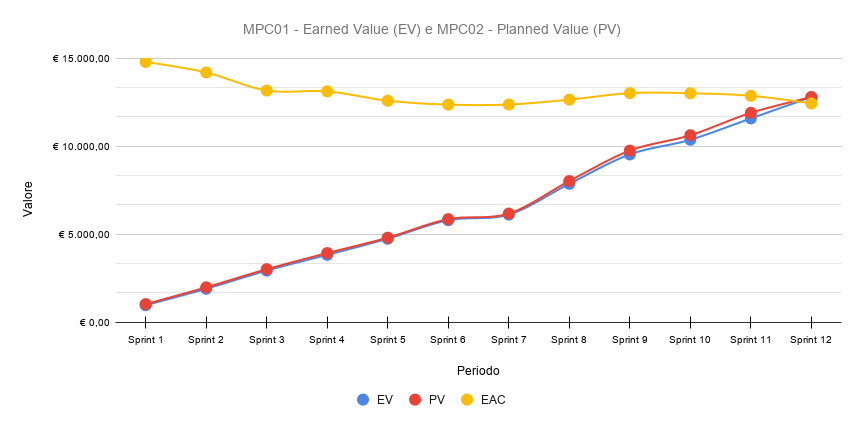
\includegraphics[width=0.9\textwidth]{grafici/MPC01_02.png}
     \caption{Grafico per periodo di MPC01 e MPC02}
 \end{figure}

\subsubsubsection{RTB\G}
L'andamento del Valore Guadagnato (\textit{Earned Value} - EV)\G risulta costantemente allineato a quello del Valore Pianificato (\textit{Planned Value} - PV)\G per tutto il periodo analizzato. Questa sovrapposizione indica l'assenza di scostamenti critici a livello di schedulazione e di scopo: il valore operativo prodotto dal team corrisponde a quanto preventivato nella pianificazione di base, confermando la solidità del piano di progetto\G.

\subsubsubsection{PB\G}
Durante la fase di Product Baseline (PB)\G, il Valore Guadagnato (EV)\G e il Valore Pianificato (PV)\G hanno mantenuto un allineamento pressoché perfetto, convergendo al traguardo finale nello Sprint\G 12. Ciò attesta l'assenza di deviazioni di scope\G e il rigoroso rispetto del piano di sviluppo preventivato nella precedente baseline\G.
\newpage

\newpage



\subsection{MPC03 e MPC07 - Actual cost (AC)\G e Estimate to complete (ETC)\G}
\begin{figure}[H]
  \centering
  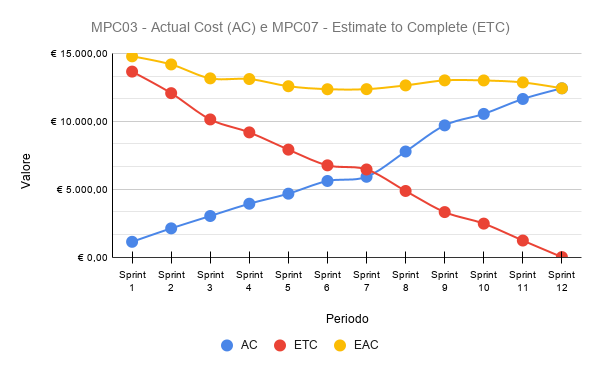
\includegraphics[width=0.9\textwidth]{grafici/MPC03_07.png}
  \caption{Grafico per periodo di MPC03 e MPC07}
\end{figure}
\subsubsubsection{RTB\G}
La metrica \textit{Actual Cost} (AC)\G registra un incremento progressivo, proporzionale all'effettivo impiego delle risorse per lo sviluppo. In modo simmetrico e inversamente proporzionale, l'\textit{Estimate to Complete} (ETC)\G decresce regolarmente. Il comportamento coerente di queste due metriche dimostra che il consumo del budget sta avvenendo in stretta correlazione con l'avanzamento dei lavori, senza generare spese impreviste o consumi anomali che avrebbero richiesto interventi correttivi.

\subsubsubsection{PB\G}
Nel periodo di PB\G, la curva dell'Actual Cost (AC)\G ha mantenuto un tasso di crescita lineare e predicibile, speculare al progressivo azzeramento dell'Estimate to Complete (ETC)\G. Il raggiungimento di un ETC\G pari a zero allo Sprint\G 12, unito a un EAC\G stabile, dimostra una corretta consuntivazione delle risorse, senza sforamenti di budget tardivi durante l'implementazione\G finale.
\newpage

\subsection{MPC04 e MPC05 - Cost Performance Index (CPI)\G e Schedule performance Index\G}
\begin{figure}[H]
  \centering
  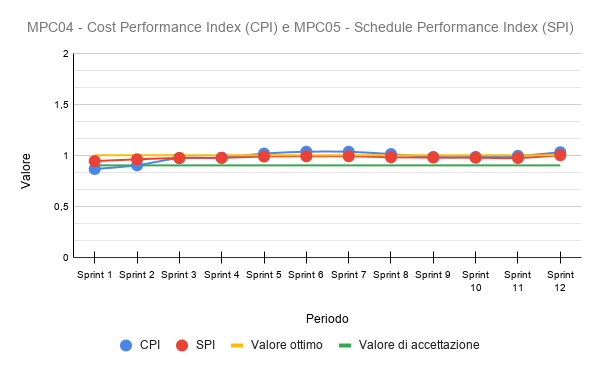
\includegraphics[width=0.9\textwidth]{grafici/MPC04_05.png}
  \caption{Grafico per periodo di MPC04 e MPC05}
\end{figure}

\subsubsubsection{RTB\G}
Nello Sprint\G 1, il \textit{Cost Performance Index} (CPI)\G si è posizionato al di sotto della soglia di accettazione (0.9) a causa dell'overhead temporale necessario per l'impostazione degli ambienti di lavoro e lo studio delle tecnologie di base. A seguito dell'introduzione di procedure di sviluppo standardizzate, l'indice è progressivamente migliorato, stabilizzandosi al di sopra del valore ottimale (1.0). Lo \textit{Schedule Performance Index} (SPI)\G si è mantenuto costantemente $\geq$ 1.0, confermando la totale aderenza alla schedulazione.

\subsubsubsection{PB\G}
Nel corso dell'intera fase di PB\G, gli indici di efficienza CPI\G e SPI\G si sono stabilizzati costantemente al di sopra del valore ottimo (1.0). Questo denota che le contromisure di processo adottate e rodate durante la fase RTB\G hanno reso il workflow\G di sviluppo pienamente maturo ed efficiente, scongiurando qualsiasi regressione prestazionale durante la scrittura del codice.
\newpage

\subsection{MPC06 - Estimated at completion (EAC)\G}
\begin{figure}[H]
  \centering
  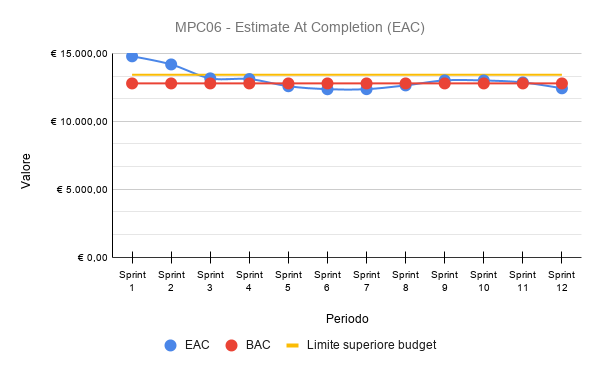
\includegraphics[width=0.9\textwidth]{grafici/MPC06.png}
  \caption{Grafico per periodo di MPC06}
\end{figure}

\subsubsubsection{RTB\G}
L'EAC\G ha inizialmente superato il budget stimato (BAC) a causa del basso indice di efficienza\G dei costi (CPI)\G registrato durante il primo sprint\G. Con l'applicazione delle azioni correttive sui processi di sviluppo, il trend dell'EAC\G si è invertito, rientrando nei limiti previsti e attestandosi in prossimità del BAC originale senza ulteriori sforamenti.

\subsubsubsection{PB\G}
L'EAC\G ha mantenuto un andamento pressochè stabile per l'intero arco temporale della PB\G, posizionandosi in sicurezza\G al di sotto del limite massimo di budget stanziato (BAC). Non si sono verificate fluttuazioni eccessive, confermando l'assoluta affidabilità\G delle stime a finire prodotte al termine della fase precedente.
\newpage

\subsection{MPC08 - Time Estimate At Completion\G}
\begin{figure}[H]
  \centering
  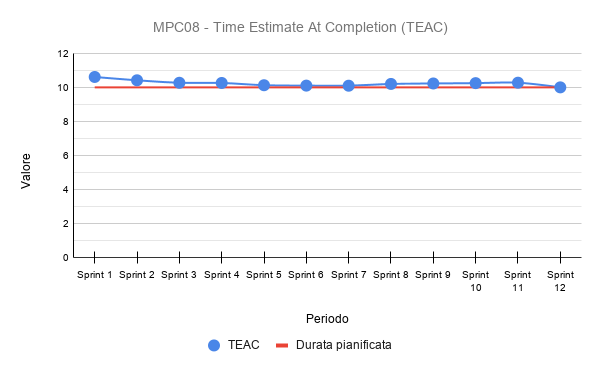
\includegraphics[width=0.9\textwidth]{grafici/MPC08.png}
  \caption{Grafico per periodo di MPC08}
\end{figure}
\subsubsubsection{RTB\G}
Il TEAC si è mantenuto costante e pari alla durata pianificata per l'intera fase RTB\G. Questo dato evidenzia l'assenza di ritardi strutturali sulla schedulazione e conferma che le variazioni registrate in altre metriche non hanno impattato la data di completamento stimata per la baseline\G in corso.

\subsubsubsection{PB\G}
Per l'intera durata della fase di PB\G, la stima temporale a finire (TEAC) si è mantenuta costantemente allineata alla durata complessiva pianificata. La totale sovrapposizione tra i tempi preventivati e l'avanzamento effettivo certifica una conduzione lineare delle attività di codifica e verifica\G.
\newpage

\subsection{MPC09 - Requirements Stability Index (RSI)\G}
\begin{figure}[H]
  \centering
  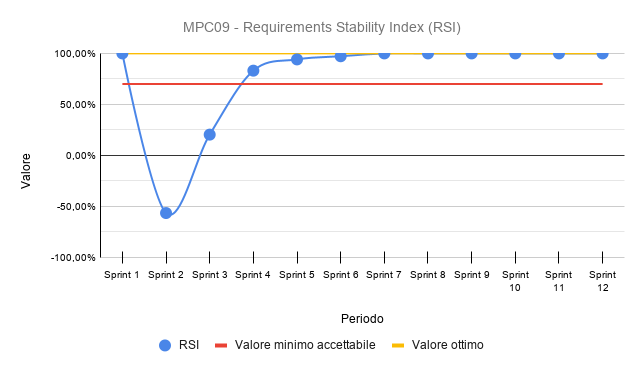
\includegraphics[width=0.9\textwidth]{grafici/MPC09.png}
  \caption{Grafico per periodo di MPC09}
\end{figure}
\subsubsubsection{RTB\G}
Nello Sprint\G 2, l'RSI\G ha registrato un valore negativo, evidenziando una forte instabilità causata da revisioni sostanziali del capitolato\G e l'emersione di nuovi casi d'uso\G. Presa coscienza di tale anomalia, il gruppo ha attuato un'azione di congelamento e formalizzazione dei requisiti. L'effetto di tale contromisura ha portato la metrica a un rapido consolidamento, raggiungendo e mantenendo il 100\% di stabilità dallo Sprint\G 5 in poi.

\subsubsubsection{PB\G}
Durante la fase di Product Baseline\G, l'Indice di Stabilità dei Requisiti (RSI)\G ha registrato un valore costante pari al 100\%. L'assenza di fluttuazioni in questo indicatore conferma oggettivamente che il consolidamento analitico effettuato al termine della fase RTB\G è stato definitivo. Il team ha pertanto condotto l'intera fase di sviluppo e implementazione\G senza incorrere in richieste di modifiche tardive, garantendo la totale integrità dell'architettura originaria.\newpage

\subsection{MPC10 - Indice di Gulpease\G}
\begin{figure}[H]
  \centering
  \IfFileExists{grafici/MPC10.png}{%
    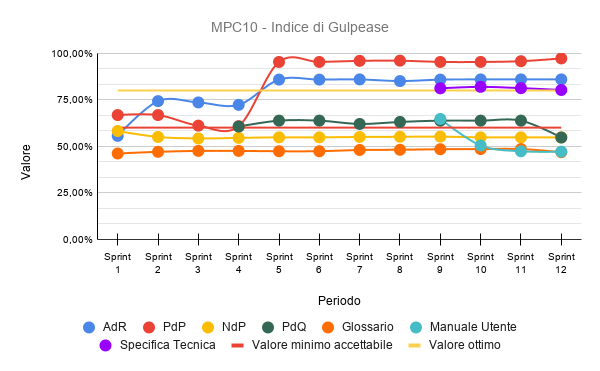
\includegraphics[width=0.9\textwidth]{grafici/MPC10.png}
  }{%
    \fbox{\parbox[c][5cm][c]{0.85\textwidth}{\centering Grafico non trovato: grafici/MPC10.png}}
  }
  \caption{Grafico per periodo di MPC10}
\end{figure}
\subsubsubsection{RTB\G}
L'Indice di Gulpease\G ha evidenziato valori sotto la soglia del 60\% per i documenti Glossario\G e Norme di Progetto\G. Questa deviazione, derivante dall'inevitabile uso di terminologia tecnica non semplificabile, è stata analizzata e accettata dal gruppo come limite fisiologico strutturale. Per la restante documentazione, in particolare per l'Analisi dei Requisiti\G, gli interventi mirati di semplificazione sintattica hanno permesso di mantenere l'indice stabilmente al di sopra della soglia ottima.

\subsubsubsection{PB\G}
Durante la fase di Product Baseline\G, l'Indice di Gulpease\G ha confermato una netta divisione strutturale. I documenti discorsivi (AdR\G, PdP\G e Specifica Tecnica\G) si mantengono stabilmente sopra la soglia ottima (80\%). Glossario\G e Norme di Progetto\G permangono sotto il minimo accettabile (60\%) per limiti terminologici intrinseci già formalmente accettati. L'unica variazione rilevante riguarda il Manuale Utente\G: introdotto nello Sprint\G 9, l'indice è sceso sotto soglia nello Sprint\G 10 a causa dell'integrazione delle sezioni tecniche di configurazione e installazione.
\newpage


\subsection{MPC13 - Quality metrics satisfied}
\begin{figure}[H]
  \centering
  \IfFileExists{grafici/MPC13.png}{%
    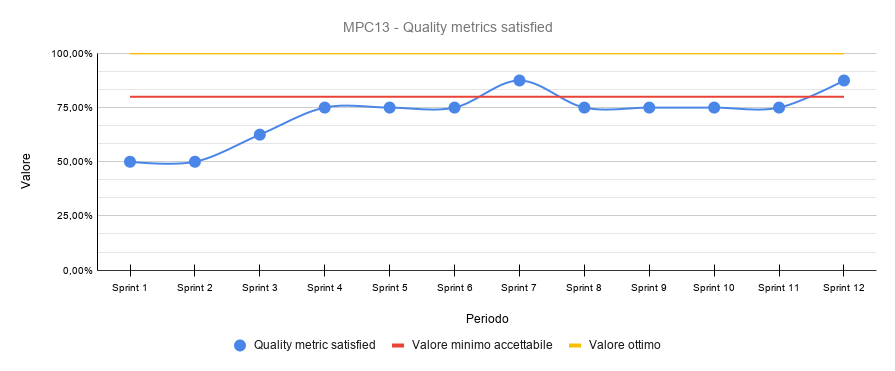
\includegraphics[width=0.9\textwidth]{grafici/MPC13.png}
  }{%
    \fbox{\parbox[c][5cm][c]{0.85\textwidth}{\centering Grafico non trovato: grafici/MPC13.png}}
  }
  \caption{Grafico per periodo di MPC13}
\end{figure}
\subsubsubsection{RTB\G}
Nei primi tre sprint\G, la percentuale di metriche soddisfatte si è mantenuta al di sotto della soglia di accettazione (80\%) a causa delle contemporanee criticità rilevate negli indici CPI\G e RSI\G. A valle dell'applicazione delle contromisure ai processi di analisi e sviluppo, l'indicatore generale è tornato a crescere. Dallo Sprint\G 4 la metrica ha superato la soglia di accettabilità, stabilizzandosi in modo permanente.

\subsubsubsection{PB\G}
L'andamento della percentuale di metriche soddisfatte durante la fase di Product Baseline (PB)\G mostra un iniziale superamento della soglia di accettazione (80\%) in concomitanza dello Sprint\G 7. Nelle iterazioni successive (Sprint\G 8-11), si è registrata una lieve flessione al di sotto del valore minimo accettabile. Tale scostamento è un indicatore fisiologico riconducibile all'emersione di difetti durante la fase di integrazione intensiva dei moduli architetturali.

\newpage

\subsection{MPC14 - Time Efficiency}
\begin{figure}[H]
  \centering
  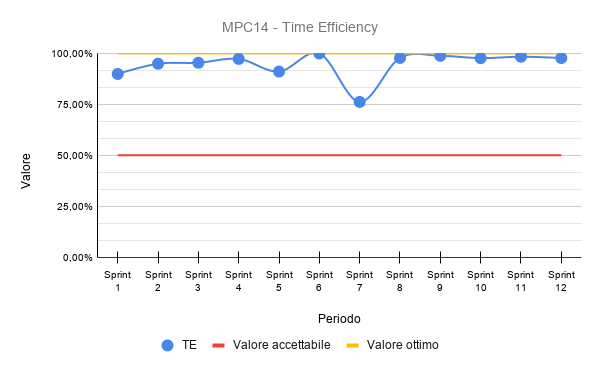
\includegraphics[width=0.9\textwidth]{grafici/MPC14.png}
  \caption{Grafico per periodo di MPC14}
\end{figure}
\subsubsubsection{RTB\G}
L'efficienza\G temporale si è mantenuta costantemente al di sopra della soglia di accettazione (50\%). Le lievi flessioni registrate negli Sprint\G 4 e 5 sono riconducibili a un fisiologico incremento delle ore di coordinamento e analisi necessarie per la riorganizzazione dei requisiti. Tali scostamenti sono stati riassorbiti nelle iterazioni successive, riportando il valore in prossimità del limite ottimo.

\subsubsubsection{PB\G}
L'efficienza\G temporale ha registrato una fisiologica flessione durante lo Sprint\G 7, in concomitanza con l'overhead strutturale richiesto per il setup architetturale e tecnologico all'inizio della fase di PB\G. Nelle iterazioni successive (Sprint\G 8-12), l'indice è rapidamente risalito stabilizzandosi su valori prossimi al 100\%, confermando il totale riassorbimento dei costi di setup iniziali.

\newpage

\subsection{MPC11 - Code Coverage\G}
\begin{figure}[H]
  \centering
  \IfFileExists{grafici/MPC11.png}{%
    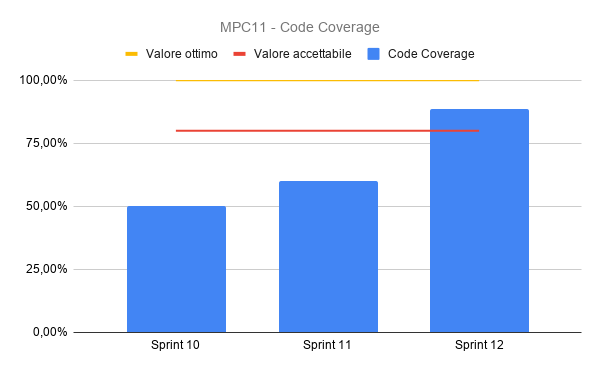
\includegraphics[width=0.9\textwidth]{grafici/MPC11.png}
  }{%
    \fbox{\parbox[c][5cm][c]{0.85\textwidth}{\centering Grafico non trovato: grafici/MPC11.png}}
  }
  \caption{Grafico per periodo di MPC11}
\end{figure}
\subsubsubsection{RTB\G}
Non sono presenti misurazioni.
\subsubsubsection{PB\G}
Negli Sprint\G 10 e 11, la \textit{Code Coverage\G} è scesa sotto la soglia di accettazione (80\%) a causa della priorità\G data allo sviluppo rapido delle funzionalità\G, che ha temporaneamente rallentato la stesura dei test\G automatizzati. Rilevato il problema, il team ha riassegnato le risorse per sanare questo debito tecnico avviando una campagna intensiva di testing. L'azione correttiva ha avuto pieno successo nello Sprint\G 12: la copertura è aumentata drasticamente superando la soglia richiesta, garantendo così l'affidabilità\G del codice per la consegna finale.
\newpage

\subsection{Esito delle misurazioni puntuali}
In questa sezione sono riportate le metriche misurate puntualmente, per le quali non è stato associato un grafico temporale. Si tratta di indicatori con valore statico, binario o calcolato su base aggregata, per cui la rappresentazione tabellare risulta più chiara e immediata.

\arrayrulecolor{primaryblue}
\begin{table}[H]
  \centering
  \begin{tabularx}{\textwidth}{|>{\raggedright\arraybackslash}p{1.8cm}|X|>{\raggedright\arraybackslash}p{3cm}|>{\raggedright\arraybackslash}p{3cm}|}
    \hline
    \rowcolor{primaryblue!40}
    \textbf{\color{white} Codice} & \textbf{\color{white} Metrica} & \textbf{\color{white} Valore accettazione} & \textbf{\color{white} Valore attuale} \\
    \hline
    MPC12 & Test\G Success Rate & 100\% & 100\% \\
    \hline
    MPD01 & Requisiti obbligatori\G soddisfatti & 100\% & 100\% \\
    \hline
    MPD02 & Requisiti desiderabili\G soddisfatti & 0\% & 0\% \\
    \hline
    MPD03 & Requisiti opzionali\G soddisfatti & 0\% & 0\% \\
    \hline
    MPD06 & Defect Density & $\leq 3$ / KLOC & 0.157 / KLOC\\
    \hline
    MPD11 & Click Count (Funzioni principali) & $\leq 5$ click & 5 click \\
    \hline
    MPD12 & User Error Rate (Errori validazione\G) & $\leq 10\%$ & 9.46\% \\
    \hline
    MPD13 & Blocker Code Smells & 0 & 0 \\
    \hline
    MPD14 & Cyclomatic Complexity\G (per metodo) & $\leq 15$ & 1.97 \\
    \hline
    MPD15 & Comment Intensity & $\geq 10\%$ & 10\% \\
    \hline
    MPD16 & Supported Browsers (Test\G passati) & 100\% (Desktop) & 100\% \\
    \hline
  \end{tabularx}
  \caption{Metriche senza grafico associato}
\end{table}






\end{document}